% Copyright 2004 by Till Tantau <tantau@users.sourceforge.net>.
%
% In principle, this file can be redistributed and/or modified under
% the terms of the GNU Public License, version 2.
%
% However, this file is supposed to be a template to be modified
% for your own needs. For this reason, if you use this file as a
% template and not specifically distribute it as part of a another
% package/program, I grant the extra permission to freely copy and
% modify this file as you see fit and even to delete this copyright
% notice.

\documentclass{beamer}

\usetheme{Goettingen}

\usefonttheme{professionalfonts} % using non standard fonts for beamer
\usefonttheme{serif} % default family is serif
\usepackage{fontspec} % Allows font customization
\defaultfontfeatures{Mapping=tex-text,Scale=MatchLowercase}
\setmainfont{Ubuntu Light} % Main document font

\usepackage{hyperref}
\usepackage[english,spanish]{babel}

\usepackage{minted}

\usemintedstyle{friendly}

\newminted{java}{
fontsize=\small,
   gobble=4,
   frame=lines,
   framesep=2mm,
   mathescape=true,
}
\newminted{xml}{
fontsize=\small,
   gobble=0,
   frame=lines,
   framesep=2mm,
   mathescape=true,
}

\title{Curso de programación Android}

% A subtitle is optional and this may be deleted
\subtitle{T-Formación}

\author{Alejandro~Alcalde}
% - Give the names in the same order as the appear in the paper.
% - Use the \inst{?} command only if the authors have different
%   affiliation.

\institute[Estudiante de la ETSIIT] % (optional, but mostly needed)
{
  \href{http://elbauldelprogramador.com}{elbauldelprogramador.com}}
% - Use the \inst command only if there are several affiliations.
% - Keep it simple, no one is interested in your street address.

\date{\today}
% - Either use conference name or its abbreviation.
% - Not really informative to the audience, more for people (including
%   yourself) who are reading the slides online

\subject{Curso Programación Android}
% This is only inserted into the PDF information catalog. Can be left
% out.

% If you have a file called "university-logo-filename.xxx", where xxx
% is a graphic format that can be processed by latex or pdflatex,
% resp., then you can add a logo as follows:

%\pgfdeclareimage[height=0.1cm]{university-logo}{university-logo-filename}
%\logo{\pgfuseimage{university-logo}}
%\titlegraphic{
\includegraphics{university-logo-filename}}

% Delete this, if you do not want the table of contents to pop up at
% the beginning of each subsection:
\AtBeginSubsection[]
{
  \begin{frame}<beamer>{Contenidos}
    \tableofcontents[currentsection,currentsubsection]
  \end{frame}
}

% Let's get started
\begin{document}

\begin{frame}
  \titlepage
\end{frame}

\begin{frame}{Contenidos}
  \tableofcontents
  % You might wish to add the option [pausesections]
\end{frame}

% Section and subsections will appear in the presentation overview
% and table of contents.
\section{Preparando el entorno}

\subsection{Instalar eclipse y el plugin ADT}

\subsubsection{Descargar el SDK de Android y eclipse}

\begin{frame}{Descargar el SDK de Android y eclipse}{}
  \begin{itemize}
  \item {
    Eclipse IDE for Java EE Developers - \href{http://www.eclipse.org/downloads/packages/eclipse-ide-java-ee-developers/keplersr2}{\textit{enlace}}
  }
  \item {
    Descargar el SDK - \href{http://developer.android.com/sdk/index.html\#ExistingIDE}{\textit{enlace}}
  }
  \item{
    Una vez descargado e instalado eclipse, instalar el plugin ADT.
  }
  \end{itemize}
\end{frame}

\subsubsection{Instalar el plugin ADT}

\begin{frame}{Instalar el plugin ADT}{}
  \begin{itemize}
  \item {
    En eclipse ir a Help » Install New Software, Click en Add.
  }
  \item {
    En el cuadro de texto, poner un nombre (Ej. ADT Plugin) y en la url \textit{https://dl-ssl.google.com/android/eclipse/}
  }

    \begin{figure}[h]
        \centering
        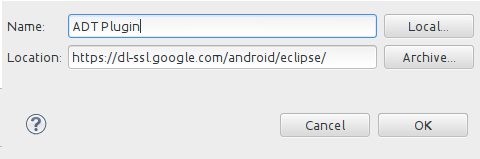
\includegraphics[scale=.5]{./img/adt.png}
    \end{figure}

    \item{A continuación, instalar las herramientas de desarrollador}

    \begin{figure}[H]
    \centering
    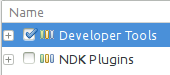
\includegraphics[scale=.4]{./img/dt.png}
    \end{figure}

  \end{itemize}
\end{frame}

\begin{frame}{Instalar el plugin ADT}{}
  \begin{itemize}
  \item {
    Una vez instalado el plugin y reiniciado eclipse, hay que decir dónde se encuentra el SDK.
  }
  \item {
    Window » Preferences » Android » SDK Location
  }
  \item{
    Instalar una imagen de Android y algunos paquetes extra.
    Window » Android SDK Manager
  }
  \begin{figure}[H]
    \centering
    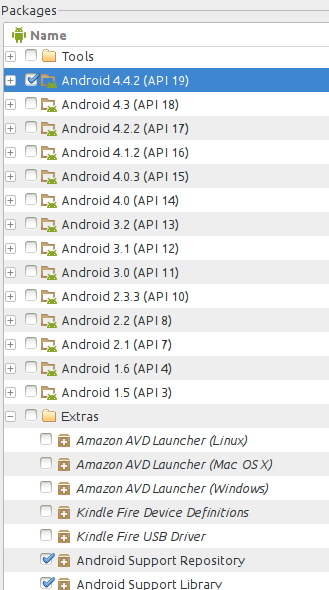
\includegraphics[scale=.25]{./img/sdkmanager.png}
    \end{figure}
  \end{itemize}
\end{frame}

\subsection{Conceptos básicos Android}

% You can reveal the parts of a slide one at a time
% with the \pause command:
\begin{frame}{Conceptos básicos Android}
  \begin{itemize}
    \item {\textbf{View:} Representa el componente básico en el que se apoyan todos los elementos que construyen una interfaz. Todos los elementos que generan interfaces heredan de la clase \texttt{\href{http://developer.android.com/reference/android/view/View.html}{View}}
    \pause
    }

  \item<2-> {
    \textbf{Activity:} Encargada de mostrar la interfaz de usuario e interactuar con él. Responden a los eventos generados por el usuario (pulsar botones etc). Heredan de la clase \href{http://developer.android.com/reference/android/app/Activity.html}{\texttt{Activity}}.
  }
  \item<3-> { \textbf{Services:} No tienen interfaz visual y se ejecutan en segundo plano, se encargan de realizar tareas que deben continuar ejecutandose cuando nuestra aplicación no está en primer plano. Todos los servicios extienden de la clase \texttt{\href{http://developer.android.com/reference/android/app/Service.html}{Service}}
  }
  \end{itemize}
\end{frame}

\begin{frame}{Conceptos básicos Android}
  \begin{itemize}
  \item{
    \textbf{Content Provider:} Ponen un grupo de datos a disposición de distintas aplicaciones, extienden de la clase ContentProvider para implementar los métodos de la interfaz, pero para acceder a esta interfaz se ha de usar una clase llamada ContentResolver.
    \pause
  }
  \item<2-> {
    \textbf{BroadcastReceiver:} Simplemente reciben un mensaje y reaccionan ante él, extienden de la clase BroadcastReceiver, no tienen interfaz de usuario, pero pueden lanzar Actividades como respuesta a un evento o usar NotificationManager para informar al usuario.
  }
  % or you can use the \uncover command to reveal general
  % content (not just \items):
  \item<3-> {
    \textbf{Intent:} Permite realizar la comunicación y transferencia de datos entre objetos de la clase Activity o Service. También permite iniciar otras Activities o lanzar otras aplicaciones.
  }
  \end{itemize}
\end{frame}

\section{Hola Mundo}

\subsection{Crear el proyecto}

\begin{frame}{Crear el proyecto}
\begin{block}{Pasos a realizar}
En eclipse, File » New » Android Application Project. Rellenamos la ventana con los siguientes datos:

\begin{figure}[H]
\centering
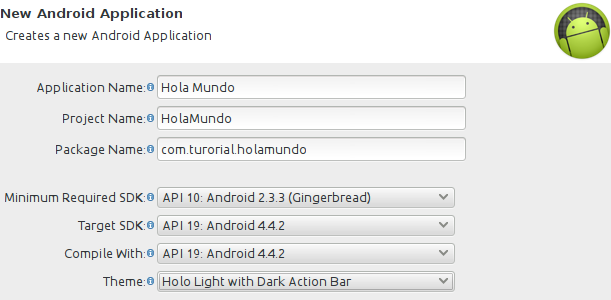
\includegraphics[scale=.25]{./img/holamundo.png}
\end{figure}
Todo siguiente hasta crear el proyecto.
\end{block}
\end{frame}

\subsection{Componentes del proyecto}

\begin{frame}{Componentes del proyecto}
\begin{block}{}
Los proyectos de Android siguen una estructura fija de carpetas que debemos respetar. Podemos ver esta estructura con la vista Package Explorer que proporciona eclipse. (En Android Studio cambia). Gen » Generados por el compilador. Assets » Recursos externos que podamos necesitar, mp3, xml etc. Res » Recursos de la aplicación (Compilados)
\begin{figure}[H]
\centering
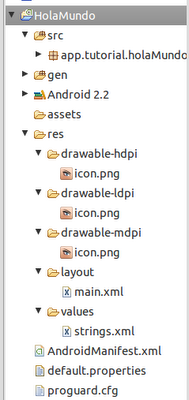
\includegraphics[scale=.3]{./img/estructuraCarpetas.png}
\end{figure}
\end{block}
\end{frame}

\subsubsection{Carpeta Res}

\begin{frame}{Carpeta Res}
\begin{block}{}
Ésta es una de la carpeta que más se va a usar junto con \texttt{src}. Se compilar y se generan referencias en la clase \texttt{R}, para acceder a ellos desde código. Están escritos en \texttt{XML}.
\pause
\end{block}
\begin{itemize}
    \item<2-> \texttt{anim}: Definición de Animaciones.
    \item<3-> \texttt{color}: Definición de colores
    \item<4-> \texttt{drawable}: Ficheros bitmap(.png, .9.png, .jpg, .gif) o XML con contenidos que se dibujarán (fondos, botones etc).
    \item<5-> \texttt{layout}: Definen la capa de interfaz de usuario
    \item<6-> \texttt{menu}: Definición de los menús de la aplicación
    \item<7-> \texttt{raw}: Binarios que no se pueden colocar en las otras carpetas.
    \item<8-> \texttt{values}: Definición de estilos, cadenas de texto para Localización etc.
    \item<9-> \texttt{xml}: Ficheros XML que pueden ser accedidos en tiempo de ejecución
\end{itemize}
\end{frame}

\begin{frame}[fragile]{Hola Mundo}
\begin{block}{}
\begin{javacode}
    @Override
    protected void onCreate(Bundle savedInstanceState) {
        super.onCreate(savedInstanceState);

        /**
         * Método encargado de “inflar” la actividad.
         * Inicializar cada componente de la actividad
         * con su correspondiente View.
         */
        setContentView(R.layout.activity_main);
    }
\end{javacode}
\end{block}
\end{frame}

\begin{frame}{Ciclo de vida de una Activity}
\begin{block}{}
\begin{figure}[H]
\centering
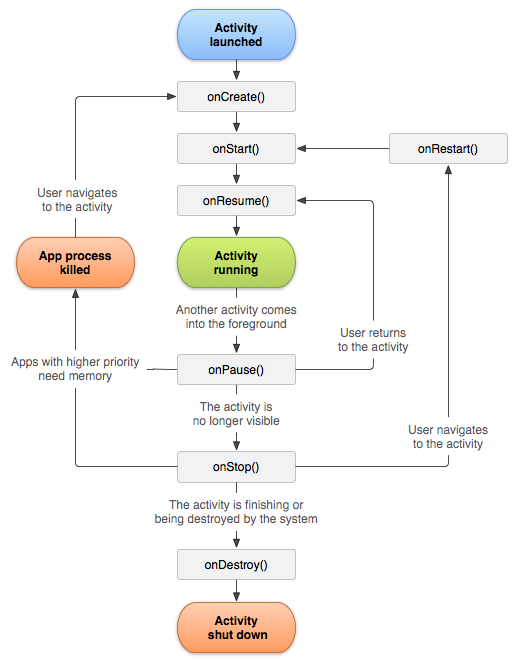
\includegraphics[scale=.33]{./img/activityLifecycle.png}
\end{figure}
\end{block}
\end{frame}

\begin{frame}[fragile]{Hola Mundo}
\begin{block}{}
\textbf{./res/layout/activity\_main.xml}
\begin{xmlcode}
<RelativeLayout
    android:layout_width="match_parent"
    android:layout_height="match_parent"
    tools:context=".MainActivity" >
    <TextView
        android:layout_width="wrap_content"
        android:layout_height="wrap_content"
        android:text="@string/hello_world" />
</RelativeLayout>
\end{xmlcode}
\textbf{./res/values/strings.xml}
\begin{xmlcode}
<resources>
    <string name="hello_world">Hello world!</string>
</resources>
\end{xmlcode}
\end{block}
\end{frame}
% Placing a * after \section means it will not show in the
% outline or table of contents.
\section*{Qué hemos visto}

\begin{frame}{Qué hemos visto}
  \begin{itemize}
  \item
    Cómo preparar el entorno para desarrollar aplicaciones Android.
  \item
    Conceptos básicos Android.
  \item
    Creación de un proyecto Hola Mundo.
  \end{itemize}
\end{frame}

\begin{frame}{¿Y ahora qué?}
  \begin{itemize}
  \item
    A partir de ahora, trabajaremos sobre ejemplos funcionales, deteniéndonos en las partes de código importantes para explicarlas.
  \end{itemize}
\end{frame}

% All of the following is optional and typically not needed.
\appendix
\section<presentation>*{\appendixname}
\subsection<presentation>*{Bibliografía recomendada}

\begin{frame}[allowframebreaks]
  \frametitle<presentation>{Bibliografía recomendada}

  \begin{thebibliography}{10}

  \beamertemplatebookbibitems
  % Start with overview books.

  \bibitem{ProAnd4}
    Satya~Komatineni.
    \newblock {\em \href{http://www.amazon.es/gp/product/1430239301/ref=as_li_ss_tl?ie=UTF8&camp=3626&creative=24822&creativeASIN=1430239301&linkCode=as2&tag=elbaudelpro-21}{Pro Android 4 - Libro en Amazon}}.
    \newblock Apress 2012.


  \beamertemplatearticlebibitems
  % Followed by interesting articles. Keep the list short.

  \bibitem{developerandroid}
    Developer.android.com
    \newblock Documentación oficial de Android.
    \newblock {\em \href{http://developer.android.com/develop/index.html}{developer.android.com}}
  \end{thebibliography}
\end{frame}

\end{document}


